\chapter{Gravitational waves}

\section{Gravitational Waves}

Gravitational waves were predicted by Einstein in his theory of \ac{GR} well over 100 years ago \cite{GR_Einstein_paper}. In his theory, Einstein shows that the more massive an object is, the greater a curvature in spacetime that object creates. This curvature can then have an effect on the motion of objects which encounter it. This is summarized succinctly by John Archibald Wheeler where he states that ``Spacetime tells matter how to move; matter tells spacetime how to curve''. Einstein formalises the relationship between matter/energy and the curvature of space-time in his field equations as

\begin{equation}\label{eqn:FieldEquations}
    G_{\mu \nu} + \Lambda g_{\mu \nu} = \frac{8 \pi G}{c^{4}} T_{\mu \nu},
\end{equation}{}

where $\Lambda$ is the cosmological constant (scalar measurement describing the energy density of space), $g_{\mu \nu}$ is the metric which describes the geometric structure of space-time, $G$ is Newton's gravitational constant, $c$ is the speed of light, $T_{\mu \nu}$ is the stress energy tensor which describes the density, direction, flow of energy in space-time and $G_{\mu \nu}$ is the Einstein tensor defined as

\begin{equation}
    G_{\mu \nu} = R_{\mu \nu} - \frac{1}{2} R g_{\mu \nu}
\end{equation}

where $R_{\mu \nu}$ is the Rici curvature tensor which determines the degree to which matter will tend to change as a function of time (trace of the Riemann tensor) and $R$ is a real valued scalar number describing the degree of curvature. 

%
% Transition towards discussing GWs as small purturbations on the flat spacetime metric
%
The Einstein field equations described by e.q. \ref{eqn:FieldEquations} unfortunately can only be solved exactly in a limited number of situations. These situations include the Schwartzchild solution for a non-spinning singularity and the Kerr solution for a spinning singularity. If we would like to explore the behavior of more non-linear, time-dependent systems in terms of Einstein's field equations we need to put his equations into a more linear form. This can be done by describing the spacetime metric $g_{\mu\nu}$ in terms of an easy computable known solution in flat spacetime with the addition of some small perturbation.

%
% Introduce g_munu
%
It turns out that gravitational waves may be defined as small perturbations over the curved background spacetime metric $g_{\mu \nu}$. In Euclidean space, the metric (which is what allows us to compute distances or dot products between two point mass objects), is generally described by the identity matrix in Cartessian coordinates. However, in \ac{GR} we have to add the time dimension and in flat spacetime this can be described by the Minkowski metric $\bar{g}_{\mu \nu}$ (sometimes also denoted $\eta_{\mu \nu}$) as

\begin{equation}
  \bar{g}_{\mu \nu} =   \begin{pmatrix}
-1 & 0 & 0 & 0\\
0 & 1 & 0 & 0\\
0 & 0 & 1 & 0\\
0 & 0 & 0 & 1
\end{pmatrix}.
\end{equation}

Since a gravitational wave is a perturbation (or an additional curvature to the flat spacetime Minkoski metric), we can write the metric with a \ac{GW} present as  

\begin{equation}
    g_{\mu \nu} = \bar{g}_{\mu \nu}(x) + h_{\mu \nu}(x),
\end{equation}{}

where $h_{\mu \nu}(x)$ is the gravitational wave perturbation. After taking the derivative of $g_{\mu\nu}$, we then arrive at the plane wave solution for \ac{GW}s written as

\begin{equation}\label{eq:gw_plane_solution}
    h_{\mu\nu} = \textrm{Re}[A_{\mu\nu} e^{(ik_{\alpha}x^{\alpha})}],
\end{equation}{}

where $A_{\mu\nu}$ is the amplitude, $k_{\alpha}$ is the wavevector and $x^{\alpha}$ is position in spacetime. Equation \ref{eq:gw_plane_solution} can be seen to have properties similar to that of an \ac{EM} wave which is typically generated by accelerating charges. However, some major differences are that a \ac{GW} is generated by accelerating masses which produce higher order quadropole (or multipole) moments and that they are naturally signficantly weaker than \ac{EM} waves (by 36 orders of magnitude). If we shift equation \ref{eq:gw_plane_solution} to the Transverse Traceless gauge we arrive at the \ac{GW} perturbation metric

\begin{equation}
  h_{\mu \nu} =   \begin{pmatrix}
0 & 0 & 0 & 0\\
0 & h_{+}e^{ic(z-t)} & h_{\times}e^{ic(z-t)} & 0\\
0 & h_{\times}e^{ic(z-t)} & -h_{+}e^{ic(z-t)} & 0\\
0 & 0 & 0 & 0
\end{pmatrix},
\end{equation}

where we can clearly see that a \ac{GW} signal is composed of both ``plus'' and ``cross'' polarizations orthogonal to each other. The effect that a passing \ac{GW} has on a set of freely floating test particles is illustrated in Figure \ref{fig:gw_plus_cross}. This effect on freely floating test masses is what we try to measure with the \ac{LIGO} \ac{GW} detectors. In the following subsection, I will talk about how the detectors function and detect such signals.

\begin{figure}
    \centering
    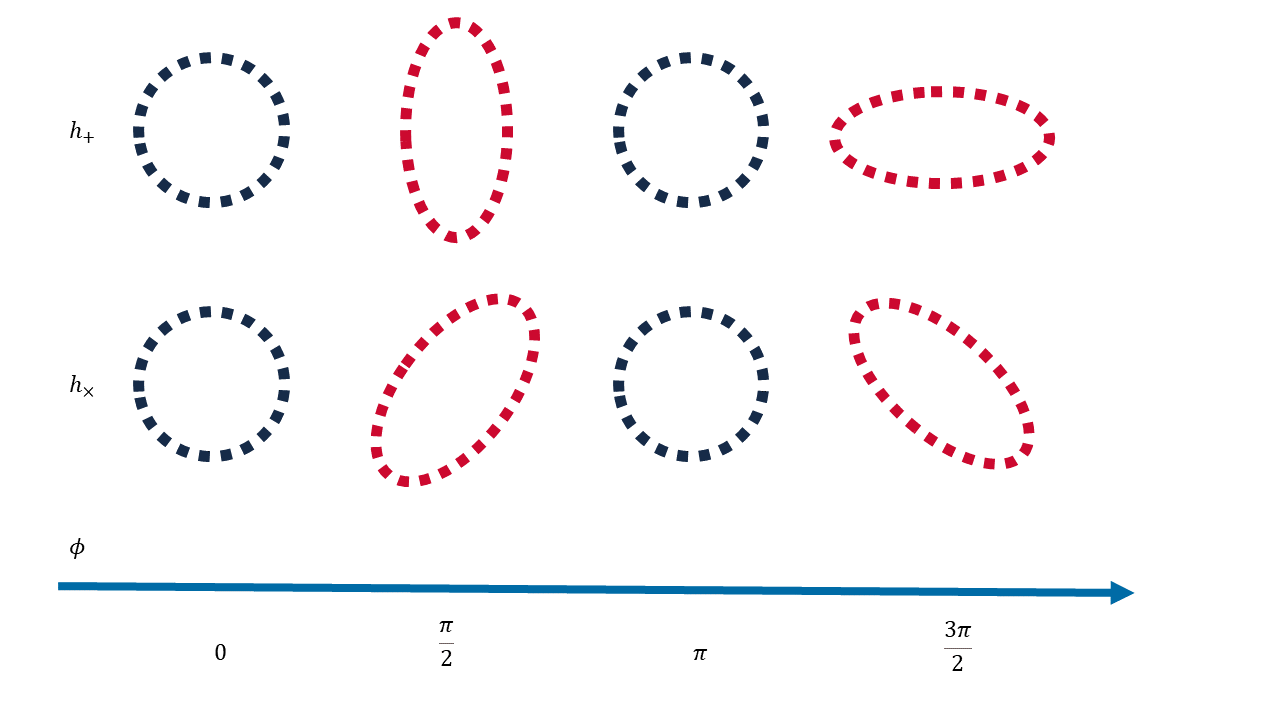
\includegraphics[width=\linewidth]{figures/GW_polarizations_thesis_figure.png}
    \caption{An illustration of the $h_+$ and $h_\times$ polarizations of a \ac{GW} signal impinging on a set of freely floating test masses as a function of phase $\phi$ from $0$ to $2\pi$.}
    \label{fig:gw_plus_cross}
\end{figure}


\section{Weber Bar Detector}

By the early 1950s technology had progressed enough such that serious 
attempts at experimentally verifying the existence of \ac{GW}s by Einstein were possible. 
One of the earliest and most well-known attempts at doing so was by 
Joseph Weber at the University of Maryland where he used an instrument 
known as a resonant-mass detector (Weber Bar Detector) \cite{PhysRevLett.18.498}. The Weber Bar 
operates on the principle that when a \ac{GW} impinges on the bar (usually 
made of some type of metal alloy, in this case high Q aluminium) it will cause 
the bar to stretch and squeeze. If the frequency of the \ac{GW} is equivalent 
to the resonant frequency of the bar, a \ac{GW} would theoretically be detectable up to a strain 
sensitivity of $h\sim10^{-16}$. Weber made the claim in 1968 that there was 
``good evidence'' for several detections made by his experiment, but unfortunately 
no others were able to reproduce his results. Although follow-up results from 
other independent studies were disappointing 
Weber's work encouraged many others to build their own improved experiments with 
breakthrough technological developments at the time and 
kick-started the subsequent field of \ac{GW} detection \cite{1009.1138}.

\section{LIGO Detectors}

%
% Could provide a bit of an introduction here, seems a bit jarring.
%

The \ac{LIGO} gravitational wave detectors are composed of 
two detectors, one in Hanford, Washington State and the 
other in Livingston, Louisiana. There are also other ground-based detectors 
in Hannover, Germany (GEO), Pisa, Italy (Virgo) and Kamioka, Japan 
(KAGRA). In addition to ground-based detectors there are eventual plans 
to build a space-based observatory called the \ac{LISA} which 
will search for super massive binary black holes (among other 
sources). Each detector can be thought 
of as a large-scale Michelson-Morley Interferometer composed 
of two arms orthogonal to each other. Each arm of 
the detectors is 4km in length. The strain a \ac{GW} induces on two free point masses 
can be expressed as 

\begin{equation}
    h(t) = \frac{2 \Delta L}{L},
\end{equation}

where $h(t)$ is the strain amplitude of the \ac{GW} 
as a function of time, $\Delta L$ is 
the relative change in length induced by the \ac{GW} on the two 
point masses and $L$ is the baseline length between the point 
masses without a \ac{GW} present. 

We record the change in length 
on the two point masses through the use of a ND:Yag 20W 
laser and large mirrors. Photons emited from the laser pass through a beam 
splitter and down the two arms of the detectors. The 
photons then hit end test mass mirrors at both ends 
and are then caught in a Fabry-Perot signal recylcing 
cavity in order to effectively increase the baseline 
length of the arms. Eventually, some photons are released 
from the Fabry-Perot cavities and return to the beam splitter 
and are recorded on a set of photodiodes which measure 
the phase difference between photons from both 
arms.

\begin{figure}
    \centering
    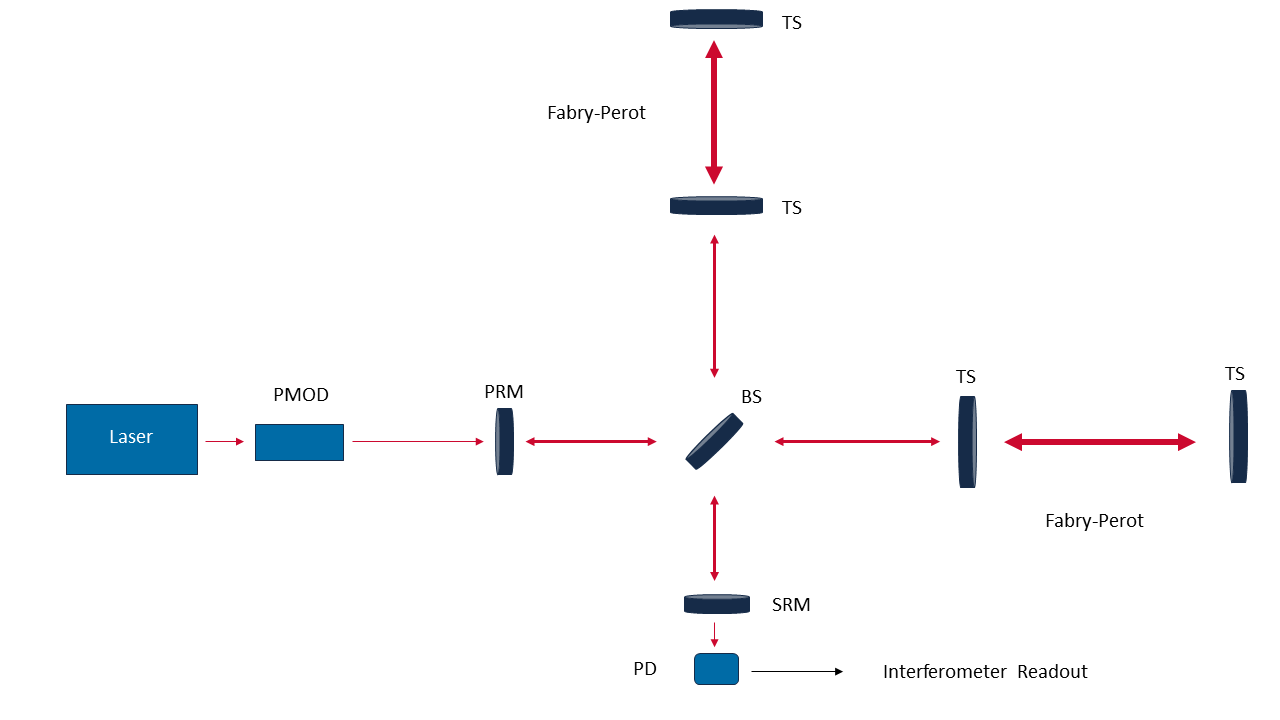
\includegraphics[width=\linewidth]{figures/Interferometer_sketch_figure.png}
    \caption{An illustration of the \ac{LIGO} detectors. A 1064nm laser beam is emited from a laser on the left-hand side, it then passes through a phase modulator (PMOD) and enters the power recycling cavity (PRM), this effectively boosts the power of the signal. The laser then passes through a beam splitter (BS), which splits the laser beam path into two seperate parts. Each part travels through an input test mass and hits end test masses at the end of both interferometer arms. The beams are then caught in a Fabry-Perot cavity which acts to extend the distance traveled of the beams, as well as the power. In other words, the cavity ``stores'' the photons for a long period ($\sim1$ ms) which allows a potential \ac{GW} signal more time to interact with the photons, thus increasing the sensitivity of the interferometer at low frequencies. Some laser light escapes back down both arms and recombines at the BS where the recombined beam passes through a signal recycling mirror (SRM). Finally, the beam hits a set of photodiodes (PD) which produce the interferometer readout which we use to determine whether or not a \ac{GW} signal is present.}
    \label{fig:gw_plus_cross}
\end{figure}


Through some algebraic manipulation we can get an estimate on the 
light travel time difference between the two interferometer 
arms as 

\begin{equation}
    \Delta \tau(t) = h(t) \frac{2L}{c} = h(t) \tau_{rt0}.
\end{equation}

%
% Need to figure out what tau rt0 is ...
%
where $\tau_{rt0}$ is the return trip time down 
one arm and the phase difference being 

\begin{equation}
    \Delta \phi(t) = h(t) \tau_{rt0} \frac{2\pi c}{\lambda}.
\end{equation}

Here we can clearly see that the phase difference 
between the two light signals is scaled by the 
length of the interferometer arms $L$. Because the 
detectors are tuned such that the photons arriving 
back at the beam splitter act to destructively 
interfere with each other, there should theoretically 
be no signal hitting the photodiodes in nominal operating times. When a \ac{GW} 
impinges on the detector, it will compress one arm 
while stretching the other arm. There will then be a 
noticeable difference in phase between the light traveling 
down both arms. Because of this difference in phase, the 
light recombining at the beam splitter will no longer 
destructively interfere and a signal will appear 
on the photodetectors.

% LIGO antenna patterns
\begin{figure}
    \centering
    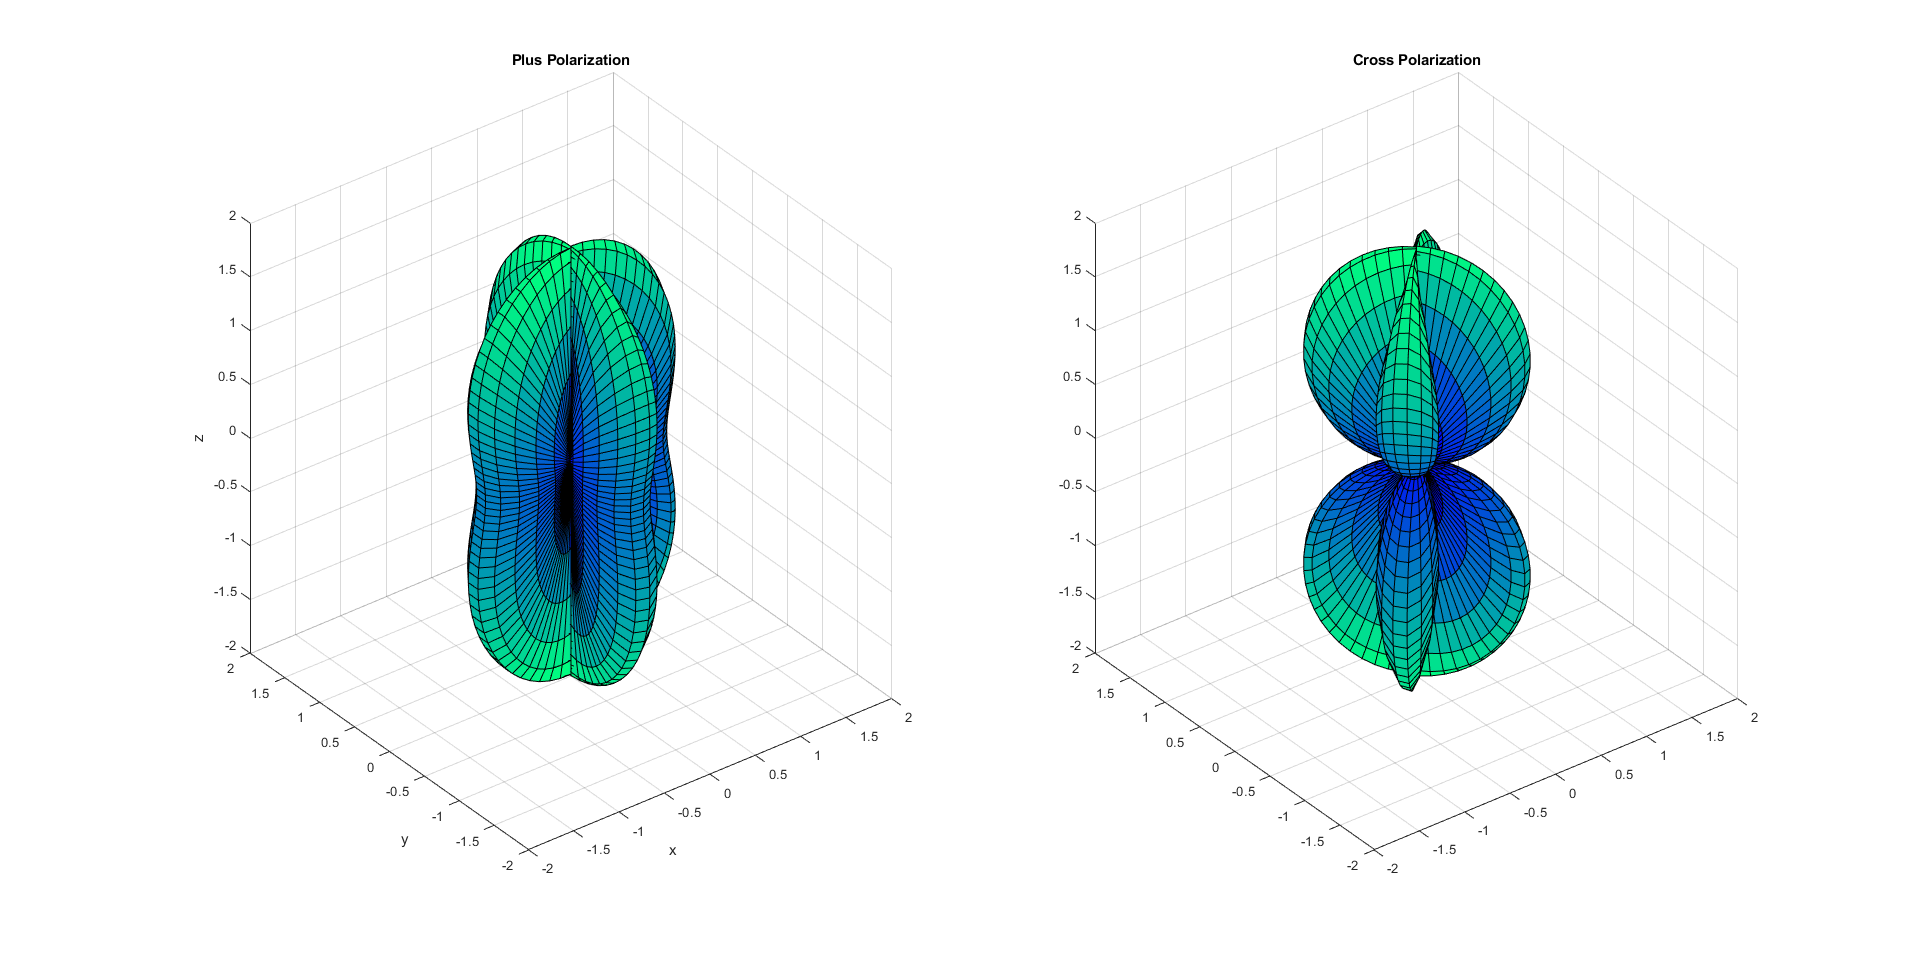
\includegraphics[width=\linewidth]{figures/peanut.png}
    \caption{An illustration of the \ac{LIGO} antenna patterns for both the $h_\times$ and $h_+$ \ac{GW} polarizations. The detector itself would lie in the x-y plane with one arm along the x-axis and the other along the y-axis.}
    \label{fig:gw_plus_cross}
\end{figure}

\subsection{Detector noise}

Although this change in phase between 
the two detector arms can be measured through 
photon counting, the detectors are 
also sensitive to non-astrophysical noise 
sources. These noise sources can drastically affect 
the sensitivity of the detectors and may also mimic 
gravitational wave events. Some common noise sources 
include anthropgenic noise, quantum shot noise, 
seismic noise and thermal noise. 

\begin{figure}
    \centering
    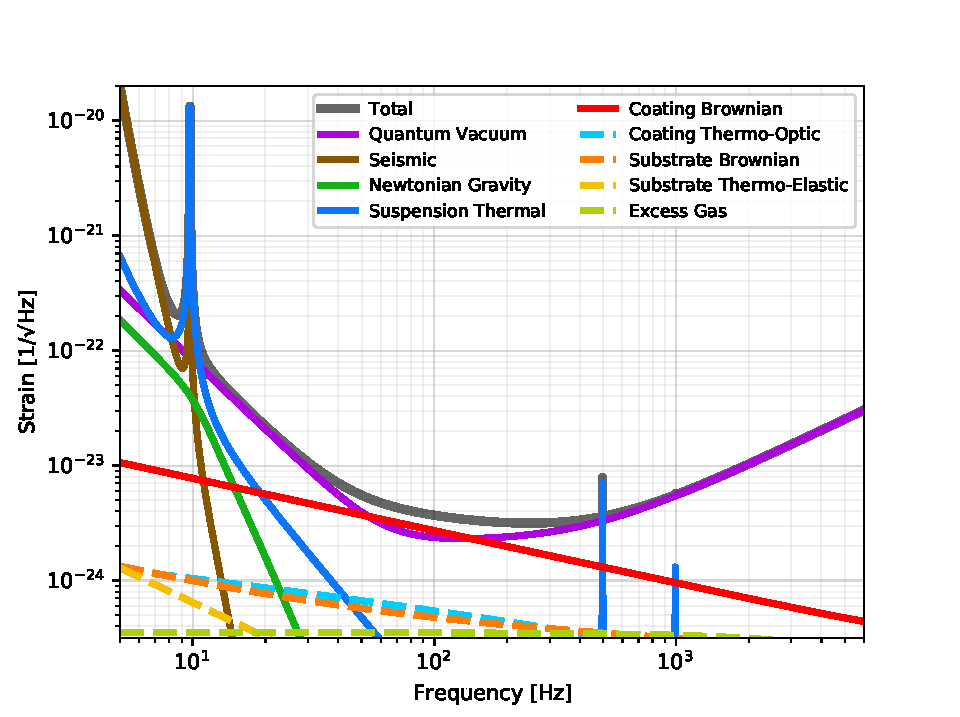
\includegraphics[width=\linewidth]{figures/aLIGO_noise_budget.pdf}
    \caption{The theoretical design sensitivity noise budget curves for Advanced \ac{LIGO}. As can be seen in the illustration, lower frequencies are largely dominated by seismic motion, mid-range frequencies thermal Brownian motion on the mirrors and higher frequencies quantum vacuum shot noise. Plot was generated using the \texttt{pygwinc} computing package \cite{pygwinc}. }
    \label{fig:gw_plus_cross}
\end{figure}

\subsubsection{Seismic noise}
Seismic noise largely affects the sensitivity of 
the detectors in the low frequency regime where 
an earthquake produces sets of waves which travel both 
through the earths core/mantel and also along the 
surface of the earth. When one of these seismic waves 
hits the detectors it can knock the interferometer arms 
out of alignment. Closely related to seismic noise 
(though at different frequencies) anthropogenic noise 
can result from individuals walking around in the 
\ac{LIGO} control rooms or large trucks passing 
on a nearby highway.

%
% Not sure if this is right. 
%
\subsubsection{Thermal noise}
Thermal noise results from the heat produced by 
the lasers passing through large coated mirrors in 
the interferometer. When laser photons pass through 
these mirrors, the photons subsequently heat up 
the coating/mirror material. This heat causes the molecules 
which make up the coating/lens material to behave in 
random Brownian motion, thus causing the photons to deviate from 
their intended path.

\subsubsection{Quantum shot noise}
Quantum shot noise results from the wave packet-like 
behavior of light as it travels through a medium. 
Because of Poisson statistics, we know that the 
uncertainty on the number of photons that we 
count arriving at the \ac{LIGO} photodiodes 
after recombination at the beam splitter is 
proportional to the expected number of photons 
arriving each second. The greater the power 
of the laser, the greater the quantum shot 
noise at higher photon frequencies.

%%%%%%%%%%%%%%%
%%%%%%%%%%%%%%% 
%%%%%%%%%%%%%%% 
\section{LIGO sources}

There are a variety of events which can cause significant 
enough distortions in spacetime to produce 
\ac{GW} events. Such events include \ac{CBC} signals, burst events,
continuous \ac{GW}s from rotating neutron stars and 
stochastic \ac{GW}s (leftover echoes from the Big Bang). In this 
section I will describe these events and how \ac{GW}s are 
produced from them.

\subsection{Compact Binary Coalescencs}

\ac{CBC} signals arise from the collision of massive compact 
objects moving at high relativistic speeds. Such systems can 
include binary black holes, neutron star - black hole pairs, binary 
neutron stars and super massive black hole encounter events. 

As the two objects rotate about each other, energy is radiated away in the 
form of \ac{GW}s due to the asymmetric motion of the heavy objects. 
Over the course of millions of years, the two objects will 
inspiral in towards each other. In so doing the objects will 
orbit faster, peturbing spacetime to a greater degree and 
thus releasing more energy in the form \ac{GW}s. In the final few 
seconds prior to merger the objects will release a large amount of 
\ac{GW} energy collide. If the objects are binary black holes, they 
will coalesce into a single black hole which will ``ring'' for a 
short amount of time. If the objects are binary neutron stars they will 
typically collide and then produce a large supernovoe event, emiting 
a large amount of \ac{EM} light in the process (which importantly 
can be measured by other telescopes across the spectrum on Earth). 

\subsection{Continuous Waves}

\ac{CW} signals are canonically associated with spinning non-axisymmetric 
neutron stars. Other more exotic sources can result from clouds of bosons 
annihilating each around fast-spinning black holes. 
Neutron stars are the leftover cores of dead stars 
which have exploded in a supernovae and then collapsed down 
into an object roughly the mass of our sun and with a radius of a 
few km. \ac{GW} signals are produced from mass quadrupole radiation in the 
gravitational field and spinning neutron stars can cause such 
disturbances through cracking and cooling of the crust, internal non-axisymmetric 
magnetic field flows, and mountains of mass accreted on the 
surface from a larger companion star \cite{1712.05897}.

\subsection{Stochastic Gravitational Waves}
%
% Cite this living review
% https://link.springer.com/article/10.1007/s41114-017-0004-1

Although the more loud signals like GW150914 get the majority of attention these days, there are many more much quieter signals that are present in the detector data streams than are detected with usual \ac{CBC} detection techniques. To quantify this statement, we can get an exact number for the rate of \ac{CBC} binary black hole signals occurring at any given time by multiplying the local rate of \ac{CBC} binary black hole events by a comoving volume (up to a predetermined redshift). If we use a redshift of $z \sim 6$ for this calculation, we wind up with a \ac{CBC} binary black hole rate of $\sim 1$ per minute. The vast majority of these events will not lie within the detectibility band of the \ac{LIGO} detectors and will make up random (or ``stochastic'') background of events in the noise. The stochastic \ac{GW} background is not only made up of \ac{CBC} signals, but any \ac{GW} event which is low enough in \ac{SNR} to lie within the general noise background of the detectors.

This stochastic background of \ac{GW} events could provide valuable insights into fundamental physics if we were able to resolve them from the instrumental/environmental noise background of the detectors. One common example used to explain the potential significance of stochastic \ac{GW} detection is the Cosmic Microwave Background (CMB). The CMB is the leftover remnants from the Big Bang ($\sim 400,000$ years after) and is the imprint left over by photons at the moment the universe had cooled enough to allow them to travel through space. Unfortunately, we are not able to see any further back since the universe prior to this period was to hot to allow photons to travel. If we were able to resolve the stochastic \ac{GW} background we would then be able to see even further back in time, right up until the very end of inflation, which is $\sim 10^{-32}$s after the Big Bang. Such accuracy could provide new insights into the early universe, as well as key information about early astrophysical source population properties and formation mechanisms. \cite{Romano2017}
 
\subsection{Burst signals}

When a white dwarf accretes enough mass from a binary companion star such that its total mass exceeds that of Chandrasekhar limit (1.44 solar masses) it may explode in the form of a type 1a supernova. Other supernova events can occur from a variety of other sources such as a supermassive red giant star when it runs out of fuel in its core at the end of its life and implodes on itself. When a supernova occurs, it is possible that \ac{GW}s may be released in some form if the event happens in a non-symmetric manner, such as if the star is rotating at great speed with minor surface mountain distortions. Because of the complex dynamics of supernova events, it is difficult to model these events and as such commonly use what is known as an unmoddeled search to look for these events. Additionally, there is also the possibility that we may find as yet unknown types of \ac{GW} sources due to the model independent agnostic nature of this type of search \cite{Sathyaprakash2009}. 

\section{Search methods for gravitational wave signals}

In this section, I will describe several methods used by the 
\ac{LVC} to search for signals from \ac{CBC}, \ac{GW}, burst and 
stochastic \ac{GW}s.

\subsection{\ac{CW} search method}

There are estimated to be roughly $\sim 10^{8} - 10^{9}$ neutrons stars 
in our own Milky Way Galaxy, of which only $\sim 2500$ have already 
been observed by the wider scientific community. One method for detecting 
\ac{CW} signals is to go after these already known $2500$ neutron 
stars and perform a targeted search.

\subsubsection{Targeted search}
The GW strain given by a non-axisymmetric spinning neutron star 
is typically defined by 

\begin{equation}
    h_{0} = \frac{4\pi^2G}{c^4} \frac{I_{zz} f^2}{d} \epsilon,
\end{equation}

where $I_{zz}$ is the moment of intertia around the z-axis of the 
neutron star, $f$ is the \ac{GW} frequency (roughly proportional to 
the star spin frequency) and $\epsilon$ is the elipticity. In a targetted 
search, we generally assume that the sky position, frequency, spin and 
other parameters are well known. There is also a middle-ground option of 
performing a directed search where we only assume to know the sky location 
very well. Nominally, a \ac{FFT} is first performed on the 
data afterwhich a transformation of some sort is then applied (
frequency-Hough, ``stack-slide'', PowerFlux) in order to 
map the observed data to source properties. After this mapping performed, 
we essentially then try to look for excesses in power above 
a pre-defined threshold over a large number of frequency bins. The 
methods listed above put many different spins on this\cite{PhysRevD.90.042002}.

\subsubsection{All-sky search}

\subsection{Burst search method}

As mentioned previously, burst-like signals are typically not modeled due to the complicated nature of the event and the possibility of detecting as yet unknown signals. Because of the uncertainty in trying to search for this type of signal, we use an unmodelled search which essentially trying to distinguish between unknown signal and noise. Since the search is unmodelled we don't necessarily have a set of template waveforms which are exactly described by a deep knowledge of numerical relativity, post-Newtonian dynamics or \ac{GR}. Rather, members of the \ac{LIGO} burst search team use template waveforms which roughly imitate events of varying statistical properties who have bursts of excess power for a short duration of time. Some of the signal template types include but are not limited to:

\begin{itemize}
    \item White Nosie burst: A signal which is of zero value and then jumps up to a predefined value in a step-like fashion before sharply falling back down to zero in a step-like fashion.
    \item String cusp: A delta-like function which is meant to mimic \ac{GW}s from cosmic string cusps.
    \item Sine-Gaussian: A sinosoidal waveform which increases exponentially in amplitude, peaking, and then subsequently decreasing exponentially in amplitude. This is meant to mimic the \ac{GW}s from a ringdown-like event.
\end{itemize}

%
% Actual burst method
%

Once we have our template bank, the first step of the burst search pipeline is to identify candidate transient events to set aside for further analysis. This is done using the WaveBurst algorithm which tries to identify clusters of times in the data stream which are coincident with each other. The coincidence is determined by times of excess power in the detector, identified through a linear wavelet packet decomposition. This process is done at several different frequency resolutions in order to not miss any features at specific frequency bands. If there is a cluster of times which are identified as having a significant amount of excess power, we then check for whether or not a similar cluster is also present across other detectors which were operational at the time. The significance of the burst-like candidate event is determined by essentially computing the geometric average of the excess signal power across all detectors in multiple frequency bins (with respect to the background noise). There are further complications which may be added to the method described above, but the reader may find more information on more robust signal consistency/coincidence methods in the following manuscript \cite{Abbott_2007}. The Burst search is currently verified for accuracy by injecting signals using the template bank described above.

\subsection{Stochastic search method}

%
% Intro to cross correlation
% Will want to rephrase the lisa null combinations phrase since it's too 
% similar to what you are citing.
The stochastic search method largely involves attempting to piece out \ac{GW} stochastic noise from the detector environmental/non-astrophysical noise. We do this by using a method known as cross-correlation analysis. Cross correlation is essentially a (sliding) dot product between two vectors of numbers, where we observe peaks in the dot product where the series are most similar. For \ac{LIGO} we look for cross correlations across multiple detectors. In \ac{LISA} we have to use special null combinations of the data where the \ac{GW} signal is suppressed enough to where there is nearly only detector noise present in the data stream. The suppression is possible to do through the symmetrized Signac method \cite{PhysRevD.64.062002}. If this can be done, one can then do an excess power measurement in order to see if there is a signal present in the noise. Alternately, it may also be useful to have a solid understanding of how to model the noise in the \ac{LISA} detectors in order to distinguish between \ac{GW} signal and noise. 

Normally, it is nearly impossible to distinguish between detector noise and the stochastic \ac{GW} background in a single detector, which is why we look for correlations between data across multiple detectors. This is made under the assumption that instrumental noise is not correlated between multiple detectors. It turns out that if we take the expected value of the cross correlation of the data between two detectors, we end up with the the variance of the stochastic \ac{GW} signal (since it is by definition supposed to be present in the data of both detectors).

%
% Frequentist vs. Bayesian approach for stochastic search
%
In order to get a more rigorous statistical estimate of the cross correlation value, one can use a number of frequentist and Bayesian approaches. The frequentist approach involves using a maximum likelihood ratio to compare two models. The two models being a noise+signal model and a noise-alone model. The frequentist approach then computes the maximum likelihood value for both models and estimates a ratio between the two values (divide the maximum likelihood estimate of the signal+noise model by the likelihood estimate of the noise model). The likelihood function which is normally used is a Gaussian multivariate function.

The Bayesian approach again use the likelihood function for each model described above, but additionally need the joint prior probability distributions for both the signal and noise parameters. A flat prior is usually used for the signal variance and Jeffrey’s prior is used for the noise variance. One can then construct a join posterior probability distribution for each model in order to figure out the likelihood of signal being present in the noise. We can quantify this exactly by computing the Bayes factor between the signal+noise model and the noise alone model.


%
% Cite this living review: https://link.springer.com/article/10.1007/s41114-017-0004-1
%



\subsection{\ac{CBC} search method}

The output of the \ac{LIGO} gravitational wave detector is a time series produced by the resulting phase shift of two lasers after recombination on a photodiode. Because our detector is not perfectly isolated from all non-astrophysical sources, the output of the detector will be a function of both a gravitational wave impinging on it, as well some noise

\begin{equation}
    s(t) = h(t) + n(t),
\end{equation}{}

where $h(t)$ is the combined strain from a gravitational wave induced on the interferometer and $n(t)$ is the noise contribution. We generally assume that the noise is both stationary and Gaussian, although in reality the detector noise can be non-Gaussian. For those cases where we have non-Gaussianity we run various glitch identification tools and techniques to identify problematic areas of the detector data output. 

Assuming Gaussian noise, our problem then becomes, how does one distinguish noise from actual signal? Fortunately, the problem of extracting low \ac{SNR} signals from the background is not uncommon in physics and the field of statistics and may be accomplished through a technique known as matched template filtering.

\subsection{Matched template filtering}

Given the current level of sensitivity of the detectors, we will be dealing within a regime where the \ac{GW} signal we are trying to detect will often be burried far below the overall background of the detector noise. Within the context of \ac{CBC} signals, it is known that as two compact objects inspiral in towards each other that both the frequency and strength of the resultant \ac{GW} signal increases with time. We can take advantage of the fact that we generally have a good understanding of the form of $h(t)$. If we know exactly the form of $h(t)$, we may construct a simple filtering technique whereby we multiply the output of the detector $s(t)$ by $h(t)$ and integrate over some observation time. We can describe the noise contribution to the noise-free signal $h(t)$ as 

\begin{equation} \label{eq:noise_contrib}
    \frac{1}{T} \int_0^T dt n(t) h(t) \sim (\frac{\tau_{0}}{T})^{(1/2)} n_{0} h_{0}.
\end{equation}{}

In E.q. \ref{eq:noise_contrib} we see that as we increase the observation time $T$, we see that the overall value of the function tends to zero. So, given enough observation time, we can effectively filter out the contribution from the noise. The keen reader will spot one issue. Given that we may not have an infinite amount of observation time due to the duty cycle of the detectors and the fact that amplitude of the gravitational wave signal is not constant as a function of time, how can we make this filtering technique more optimal given finite observation time $T$. We define an optimal signal-to-noise ratio

\begin{equation}
    SNR_{opt} = 4 \int_0^{\infty} df \frac{|\bar{h}(f)|^2}{S_{n}(f)},
\end{equation}{}

where $|\bar{h}(f)|^2$ is is the inner product of the ideal signal template with itself and $S_{n}(f)$ is the single-sided noise \ac{PSD}. In matched template filtering, we generate many thousands of templates and compute the optimal \ac{SNR} of each. The best matching will contain the highest optimal \ac{SNR} for that event. If the \ac{SNR} is above the detection threshold (usually defined as 8), we say that there is a candidate gravitational wave signal present in the data.

%
% chi squared test
%
Because the \ac{LIGO} detectors can sometimes have non-Gaussian noise artefacts, these ``glitches'' can mimic high \ac{SNR} events. The high \ac{SNR} glitch events typically contain lots of power within a very small frequency band, distinguishing themselves from \ac{GW} events. To quantify the likelihood of a candidate high \ac{SNR} event being a real \ac{GW} signal, we use a statistic known as the chi-squared test. Specifically, the chi-squared test checks the statistical differences between the distribution of power across a set number of frequency bins in the observed data with frequency bins from the template which has been determined to match best with the data according to the matched template filtering algorithm.

Frequency bins are chosen such that each individual bin contributes an equal amount to the total matched filter \ac{SNR}. The Pearson chi-squared statistic is defined as 

\begin{equation}
    \chi^2 = \sum_{i=1}^{n} \frac{(O(i) - E_i)^2}{E_i} 
    = N \sum_{i=1}^{n} \frac{(O(i)/N - p_i)^2}{p_i},
\end{equation}

%
% Really need to figure out what p_i actually is
%
where $\chi^2$ is a finite value which determines how well your observations $O$ match your expected values $E$, $N$ are all your frequency bins, and $p_i$ is the level of matching in the $i$th frequency bin. To put this in terms of \ac{GW} matched template filtering we can plug in our variables describing our observed data and expected template values into the expression to get 

\begin{equation} \label{eq:gw_chisquared}
    \chi^2 = p \sum_{i=1}^p \left[  \left( \frac{\rho_{\mathrm{cos}}^2 }{p} - \rho_{\mathrm{cos}, i}^2 \right) 
    + \left( \frac{\rho_{\mathrm{sin}}^2 }{p} - \rho_{\mathrm{sin}, i}^2 \right) \right],
\end{equation}

where $p$ are our frequency bins, $\rho_{\mathrm{cos}}$ and $\rho_{\mathrm{sin}}$ are the matched filter \ac{SNR} values of the best matching template in both polarisations. The higher the value of E.q. \ref{eq:gw_chisquared}, the less likely that the observed data matches the best matching template. The \ac{SNR} previously determined by the matched filtering algorithm is then weighted by the chi-squared value. If the weighted match filter \ac{SNR} lies below a user predefined value, the candidate event is discarded and not considered for further analyses \cite{0264-9381-33-21-215004}. The final detection statistic is the quadrature sum of the chi-squared weighted matched filter \ac{SNR} across all detectors where the event was seen.

%
% Coincidence testing
%
Furthermore, we need to ensure that events which we observe in one detector are generally consistent with what we would expect to find in other active \ac{GW} detectors around the globe. If an event has been identified in one detector, it must also appear in other active detectors within the expected window of time it would require for the \ac{GW} to travel from one detector to another (roughly equivalent to the speed of light). The amount of time varies depending on sky location of the event, but generally it is expected to arrive at another detector within 15 milliseconds (with added uncertainty due to measurement uncertainty). The same event in multiple detectors are also expected to have the same matching template from the matched filtering algorithm.

%
% Time slides
% Not sure if I'm describing time slides correctly here.
Now that we have a detection statistic in the form of the weighted quadrature summed \ac{SNR} across multiple detectors described above, we would like a method for determining the statistical significance of this statistic. This can be done by determining the false alarm rate of the detectors as a function of the weighted detection statistic. Because we don't necessarily know how the noise of the detector is going to be distributed due to the varied non-Gaussian nature of the detectors, we have to experimentally measure the false alarm rate. We can measure this through the use of time slides. Time slides are applied by computing the number of detected triggers outside of the light travel time coincidence window (15 milliseconds) for a pre determined number of observation windows. The triggers are calculated using the best matching template for the original candidate event. The time slide windows used with the best matching template, the more sensitive the estimate on the false alarm rate. The false alarm rate is then used in order to assign a p-value to the candidate \ac{GW} event.

\subsection{Bayesian gravitational wave parameter estimation}

%
% Use this reference: https://www.cambridge.org/core/journals/publications-of-the-astronomical-society-of-australia/article/an-introduction-to-bayesian-inference-in-gravitationalwave-astronomy-parameter-estimation-model-selection-and-hierarchical-models/D459F61D8C37F0BEF86D60F42A418304
%

%
% Introduce Bayes theorem
%
It is not only important that we detect a \ac{GW} event, but also that we infer the underlying properties of that event in the form of its source parameters (i.e. component mass, distance, sky location, etc.). In \ac{LIGO}, the tried and true method for inferring source parameters is done through Bayes theorem. Bayes theorem was first used by Reverand Thomas Bayes in the 18th century and in it he proposed a new paradigm for thinking about the laws of conditional probability. To describe succinctly, Bayes theorem says that one can infer the limits on an unknown parameter by computing the likelihood of a given observation and our prior belief on the distribution of the unknown parameter. To put it in the context of \ac{GW} astronomy, given an observed gravitational wave event and some prior assumptions, we would like to infer the source parameter values of that signal while also taking into account the uncertainty added by the signal being burried in noise. We call the inferred source parameters with uncertainty the posterior 

%
% Introduce posterior
%
\begin{equation}
    p(\theta | d),
\end{equation}

where $p(\theta | d)$ is the probability of the source parameters of the signal ($\theta$ being a continuous variable), given some observed data (in the form of a time/frequency series). We assume that the integral over the total posterior is normalised such that 

%
% State that posterior is normalised such it integrates to 1
%
\begin{equation}
    \int d\theta p(\theta | d) = 1.
\end{equation}

According to Bayes theorem, we can write the posterior as 

%
% Show Bayes theorem
%
\begin{equation}
    p(\theta | d) = \frac{p(d|\theta)p(\theta)}{p(d)},
\end{equation}

%
% Discussion on priors
%
where $p(d|\theta)$ is the likelihood of our observable $d$ given source parameters $\theta$, $p(\theta$) is our prior assumptions on the distribution of the source parameters $\theta$ and $p(d)$ is a normalisation factor called the evidence. The prior $p(\theta)$ is largely informed by our understanding on the formation channels of \ac{GW} sources and our level of understanding on the general physics which govern events. For example, we would intuitively think that the mass of an object should always be positive, so will set the priors such that the component masses of a \ac{GW} source must always lie between two positive values. However, if we aren't as knowledgeable about a particular parameter $\theta$, we might try choosing a relatively uninformative prior by employing something like a broad uniform distribution. Choice of prior can also be incredibly influential on the conclusions drawn on some \ac{GW} parameters such as spin. For further interesting discussions on prior choices see Salvatore et al. \cite{PhysRevLett.119.251103}.

%
% Discussion on likelihood
%
The way in which we define the likelihood $p(d|\theta)$ (our certainty on the observed data) is essentially up to the practitioner. For \ac{GW} astronomy, we define a likelihood which assumes that the detectors operate under Gaussian noise-like conditions. The Gaussian-noise likelihood function can written as 

\begin{equation}
    p(d|\theta) = \frac{1}{\sqrt{2\pi \sigma^2}} \textrm{exp}\left(-\frac{1}{2} 
    \frac{(d - \mu)^2}{\sigma^2}\right),
\end{equation}

where $\sigma$ is the detector noise, $d$ is the observed data and $\mu$ is a template \ac{GW} waveform parameterized by source parameters $\theta$. 

%
% Discussion on the evidence
%
The evidence $p(d)$ can be defined as 

\begin{equation}
    p(d) = \int p(d|\theta) p(\theta) d\theta.
    \label{eq:evidence}
\end{equation}

The evidence is usually referred to as the marginal likelihood. Because we are marginalising over all parameters $\theta$ in Eq. \ref{eq:evidence}, we can think of the evidence as essentially a normalising factor. Since the evidence is just simply a normalising factor and it is prohibitively expensive to compute this factor, most Bayesian practitioners will ignore Eq. \ref{eq:evidence} and rewrite Bayes theorem in the simpler form 

\begin{equation}
    p(\theta | d) \propto p(d | \theta) p(\theta).
\end{equation}

\subsubsection{Markov Chain Monte Carlo}

%
% Intro and Monte Carlo sampling
% Great video on this: https://www.youtube.com/watch?v=OTO1DygELpY&ab_channel=StataCorpLLC
\ac{MCMC} is usually used when we would like to try and sample from some distribution $p$, or approximate the expectation value of some function $f(x)$ which is of a high dimension/complexity. Where $p$ is so complicated that trying to sample from $p$ analytically would be prohibitively expensive. The Monte Carlo portion of \ac{MCMC} refers to a technique known as Monte Carlo sampling. Monte Carlo sampling means to randomly sample from some distribution. For example, I could choose to randomly sample from a normal distribution $N(0,1)$ or from uniform distribution between -1 and 1. We would define the normal or the uniform distribution that I'm sampling from the proposal distribution. We should see if we randomly sample from the proposal distribution enough times, that a histogram of the resulting samples should resemble that of the original proposal distribution. 

%
% Markov Chain
%
Markov Chain refers to how we are going to go about sampling from that space. Specifically, a Markov Chain is a sequence of numbers where each number in the sequence is dependent on the previous number in the sequence. For example, if we again decided to randomly sample from proposal distribution $N(0,1)$, but instead after each sample is drawn we change the mean of the proposal distribution to be equal to that of the previous sample $N(x_{n-1},1)$, we would end up with something known as a random walk. I will note hear that this approach would not necessarily reproduce the original proposal distribution.

%
% How to accept/reject proposals
%

We can use a variety of algorithms to go about deciding how exactly accept or reject new samples drawn from the proposal distribution. One common algorithm for doing so is the Metropolis-Hastings algorithm. This algorithms works by first calculating the likelihood value for the new proposed sample, as well as the likelihood value of the previously proposed sample, and then computes the ratio of these two values. If the likelihood value of the new proposed sample is greater than the old value, then we will always accept the new value. If however, the new value is not greater than the old value, then we will not necessarily discard the old value. Instead, we can treat the new proposed likelihood value as an acceptance probability. In order to determine acceptance in this case, we can draw a uniform random number between 0 and 1 and keep the new value if it's likelihood is greater than the randomly drawn number.

%
% Issues with Metropolis Hastings
%
Unfortunately there are a few downsides to using the Metropolis Hastings algorithm. One them being that we have to choose a starting point for the random walk, which is initially liable to be far from the true posterior. Thus it may take some iterations for the algorithm to walk its way towards areas of high likelihood. We can avoid this issue by discarding an arbitrary number of samples at the beginning of the walk such that the remaining represent a point after which the algorithm has reached a stable equilibrium. We call the discarded samples the burn-in period. Another issue relates to something known as autocorrelation. Predictions on parameters $\theta$ are known to be somewhat correlated with each other due to the fact that they are all generated from the same Markov process. The fact that this correlation exists is fine, but excessive correlation can mean that there are issues with the model being used. A helpful method for tempering such correlations can be through the process of thinning. Thinning involves generating a large amount of samples from the proposal distribution, but only keeping every $N^{\textrm{th}}$ sample from that large sample set. 

%
% Could be useful to make a trace plot here.
%

%
% The whole section here really needs to be rewritten so that it's actually coherent.
% see: http://www.inference.org.uk/bayesys/nest.pdf
\subsubsection{Nested Sampling}

Nested sampling is another method which can be used in order to explicitly sample from the posterior. However, that wasn't the primary goal in mind when the method was first developed and the posterior is only really obtained as a byproduct. An additional motivation for nested sampling relates to the fact that \ac{MCMC} can have issues when trying to deal with complex multi-modal and degenerate distributions, so an improved method that handles such issues was needed at the time. Nested sampling was first introduced by Skilling in 2004 because he wanted a way to go about computing the evidence (sometimes known as the marginal likelihood) in a feasible way in order to compare different models effectively. The evidence can be described as

\begin{equation}
    Z = \int p(\theta) L(\theta) d\theta \label{eq:evidence}
\end{equation}

where $p(\theta)$ is the prior distribution and $L(\theta)$ is the likelihood function. Samples from the posterior can then be obtained as a byproduct following the evaluation of the evidence $Z$. One might naively assume that it would be easy to evaluate this integral by directly computing the expression for each parameter $\theta$. Unfortunately, this procedure can get computationally expensive quickly as the number of inferred parameters $\theta$ increases. Rather than integrating over the whole space of parameters $\theta$ explicitly, it would be advantageous to redefine Eq. \ref{eq:evidence} so that it was only dependent on a single parameter and an approximate method for computing the integral could be found. The fundamental idea that a complex high-dimensional problem with many inferred parameters implies a representation in a 1-dimensional form is one of the key ideas of nested sampling. This then begs the question, how do we go about computing the evidence in a 1-dimensional way?

We can start by generating a finite lattice of points sampled stochastically from the prior distribution. These random points are colloquially known as ``live'' points. Next, we would like to design an algorithm which evolves the ``live'' points to explore the likelihood space to find the global (or at least close to global) point of maximum likelihood. Ideally we would like to draw from a prior which also decreases in size as we move into regions of the likelihood space which dominates the posterior. Theoretically, the point with the highest likelihood would have a very small region of the prior space to sample from and the point of lowest likelihood would have nearly the whole prior space to sample from. Because the prior is by definition normalised to be between $0$ and $1$ if we framed the problem such that it was likelihood as a function of prior space being sampled from, we would have a nicely behaved, smooth, monotonically decreasing function which could be integrated easily. We can start by expressing Eq. \ref{eq:evidence} as 

\begin{equation}
    Z = \sum_{i=1}^{N} L_i w_i,
\end{equation}

$L_i$ is the corresponding likelihood value of the $i$th sample and $w_i$ is a weighting term defined as

\begin{equation}
    w_i = p(\theta_i) d\theta.
\end{equation}

This weight can be thought of as the subset of the prior distribution which is represented by the $\theta_i$th sample. The total prior mass can be defined as

\begin{equation}
    X(\lambda) = \int_{L(\theta) > \lambda} p(\theta) d\theta,
\end{equation}

where $X(\lambda)$ is the prior mass distribution (a summation over the prior $p(\theta)$) and $\lambda$ is an arbitrary cutoff value. We see that as $\lambda$ increases, the enclosed prior mass $X(\lambda)$ will then decrease. Because $X(\lambda)$ must lie between 0 and 1 and is a smooth continuous function, we can rewrite the evidence integral in terms of a single variable expression which is far easier to compute than Eq. \ref{eq:evidence}

\begin{equation}
    Z = \int_{0}^{1} L dX. \label{eq:simple_evidence}
\end{equation}

The likelihood $L$ is fairly easy to evaluate for any one sample within the enclosed likelihood space $L$ 

We can explicitly evaluate the simplified evidence in Eq. \ref{eq:simple_evidence} by first drawing $N$ random points from the prior distribution $p(\theta)$. We then iterate over a pre-determined number of iterations. For each iteration we compute the likelihood of all sampled points and determine the point with the minimum likelihood value. We then compute an estimate on the difference between the amount of prior mass covered by the the current samples above and up to the minimum likelihood value sample. We call this estimate the weight $w_i$ and we increment the evidence $Z$ by $L_i w_i$. Finally, we replace the lowest likelihood point $L_i$ with a new point which is sampled through a process like \ac{MCMC}. We only need to generate one new point because we can simply reuse the remaining $N-1$ surviving points since they are all better than the lowest likelihood point. We can generate a new sample by making a copy of one of the remaining samples and then evolving that sample through an \ac{MCMC} process. Alternatively, one can also generate a new point by genetic mixing of survivor point coordinates \cite{skilling2006}.

%
% Intro to nested sampling
%

\subsubsection{Nuisance parameter marginalization}

\section{GW detections}

%
% Intro
%

Since it's inception, \ac{LIGO} has had several observing runs. 
During the first observing run, \ac{LIGO} detected a total of $3$ binary 
black hole mergers. During the second observing run \ac{LIGO} detected an 
additional $7$ binary black holes and made the very first detection of a 
\ac{BNS} event. During the third observing run the collaboration made an 
additional $39$ confirmed \ac{GW} event detections. Of those $39$, there were 
some which could not be determined whether or not they were from a \ac{BBH} 
or \ac{BNS} \cite{1811.12907, 2010.14527}. 

%
% Mention expected rate of detections
%

Going forward, as the detectors continue to be upgraded using 
the latest cryogenic and quantum squeezing technologies, it is expected 
that the sensitivity of the detectors will increase and thus also the 
rate of \ac{GW} detection. The expected rate of detection is 

\section{Multi-Messenger Astronomy}

After a \ac{GW} signal has been identified and posterior samples have 
been obtained, an alert is sent out to other \ac{EM} partners around the 
globe in order to perform follow-up analysis. Prompt follow-up analysis could 
provide new insights into fundamental astrophysical processes such as 
the neutron star equation of state and enhanced measurements on 
the Hubble Constant. Astronomical partners include instruments which look across 
the whole range of the \ac{EM} spectrum including: Radio, Microwave, 
infrared, visible light, ultra-violet, X-ray and gamma ray. A full Bayesian 
inference analysis is typically done on all viable \ac{GW} candidates, but 
in order to produce low-latency parameter estimation products we also 
use tools such as \texttt{Bayestar} \cite{2016PhRvD..93b4013S}. \texttt{Bayestar} operates under the 
assumption that a large degree of the information contained in a \ac{GW} 
signal is encapsulated within a small number of products produced by the 
search matched template filtering process, namely: the time, amplitude 
and phase of the signal. Using a simplified likelihood function and the 
Fisher information matrix, \texttt{Bayestar} is able to produce posterior 
samples on a limited number of source parameters (sky location, distance and orientation) 
in under a few minutes which provides a good approximate of the full 
Bayesian posterior.

%
% Example of GW170817 sky localization. Not sure if I'm allowed to use other people's figures
%

\begin{figure}
    \centering
    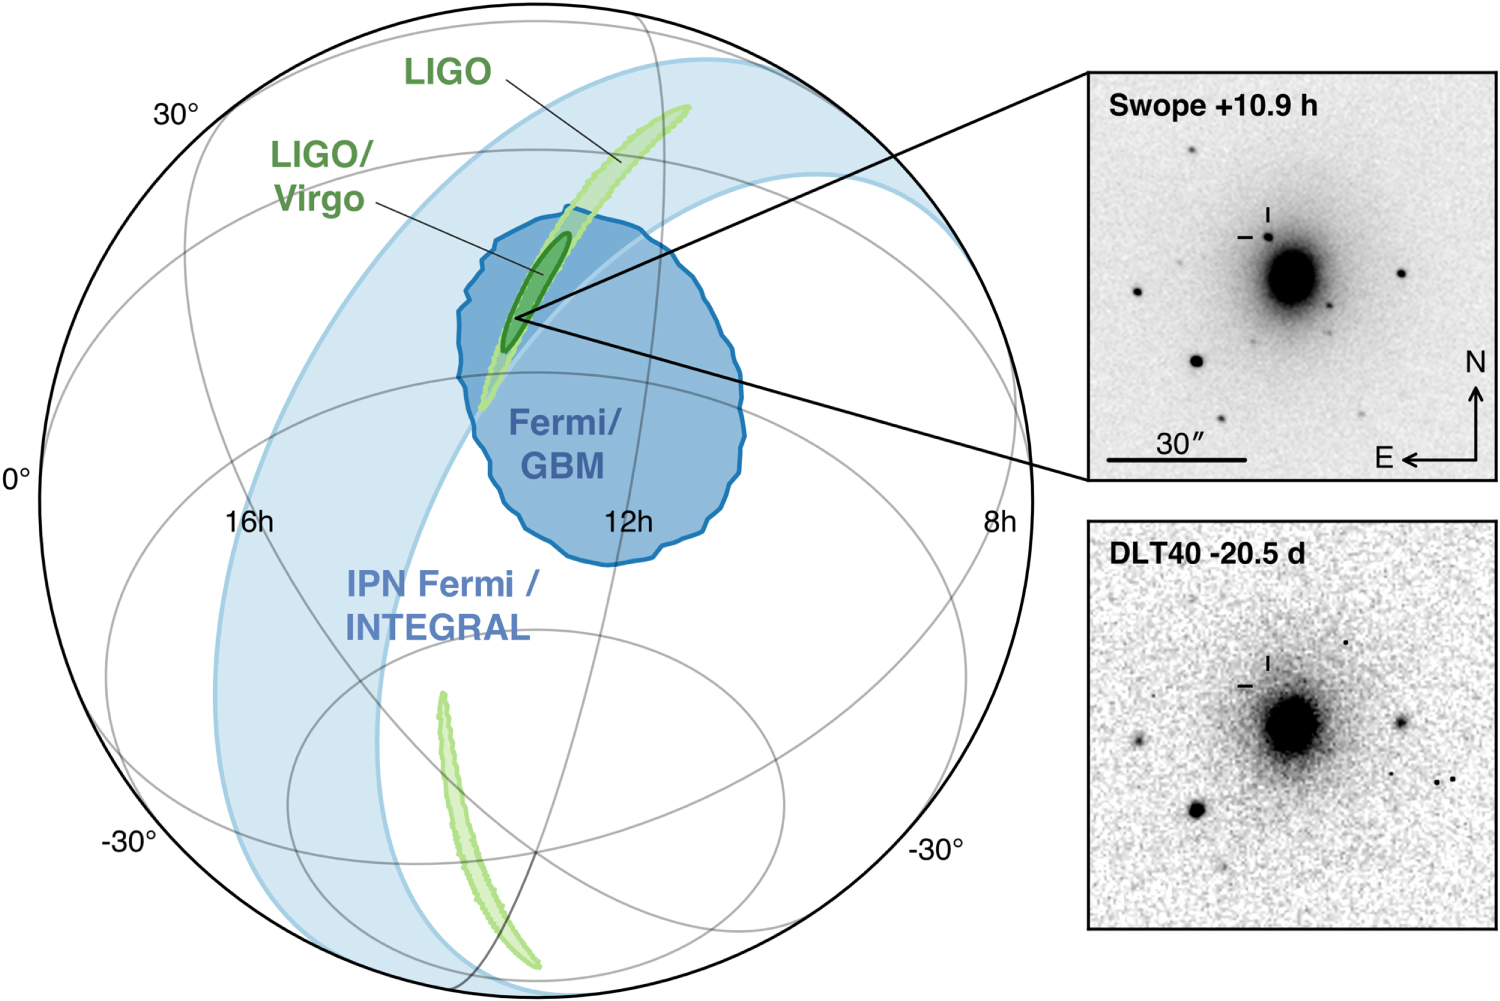
\includegraphics[width=\linewidth]{figures/GW170817_skymap.jpg}
    \caption{Sky localization for the first confirmed detection of a \ac{BNS} merger by \ac{LIGO}. Areas shaded in green are the data products from \texttt{Bayestar} using both \ac{LIGO} alone and \ac{LIGO}/Virgo combined, dark blue are predictions from Fermi/GBM and light blue are predictions from IPN Fermi/INTEGRAL. Black and white images on right-hand side are visible light measurements of a bright event around the galaxy NGC 4993 thought to contain the afterglow of the \ac{BNS} event. \texttt{This figure is was produced by the authors of the following article} \cite{2017arXiv171005833L}. }
    \label{fig:gw_plus_cross}
\end{figure}

\section{Summary}

In this chapter we provided a brief introduction to Einstein's 
Field Equations and how those field equations lead to the prediction 
that \ac{GW}s exist. We described various sources which are 
able to produce \ac{GW}s and how the \ac{LIGO} detectors physically operate 
to detect such signals. We also described the search techniques for 
all source signals and how we generate predictions on the underlying 
source parameters of \ac{GW} signals. We finally end the chapter by 
discussing multi-messenger astronomy.

